\documentclass[fleqn,10pt,a4paper,twoside,english]{book}                
%%%%%%%%%%%%%%%%%%%%%%%%%%
%% PACKAGE LOADING TIME %%
%%%%%%%%%%%%%%%%%%%%%%%%%%
\usepackage{graphicx}
\DeclareGraphicsExtensions{pdf,png,jpg}
\graphicspath{{Figures/}}

%\usepackage{pgf}
%\usepackage{lscape}
%\usepackage{pseudocode}
%\usepackage{times}      % use Times New Roman Type 1 fonts  (redefines sfdefault,rmdefault,ttdefault)
%\usepackage[T1]{fontenc}
%\usepackage{pslatex}


\usepackage{fancyhdr}
\pagestyle{fancy}
\renewcommand{\headrulewidth}{0pt} % To remove the horizontal top line from fancy page 

\usepackage[english]{babel}
%\usepackage[sectionbib,numbers,sort&compress]{natbib}  %for citations a la 'Vermeulen et al.' instead of [1]
\usepackage{tocbibind} % automatically add bibliography, list of figures, ... to table of contents
%\usepackage[a4paper,verbose, asymmetric, centering]{geometry}  % better control over margins
\usepackage[paperheight=24cm,paperwidth=16cm,verbose, asymmetric, centering]{geometry} 
%usepackage[justification=left,labelfont={bf,normalfont},textfont=normalfont]{caption} 
\usepackage[labelfont={up,bf},font=small]{caption}      %better control over captions (sideways, font, ...)  
%\usepackage{subfigure}  % with scriptsize or so, one can adapt the size - don't use together with subcaption which is better
%\usepackage{subfig}  % with scriptsize or so, one can adapt the size
%\usepackage{cite}
\usepackage{slashbox}
\usepackage{enumerate}  % to make it possible to define the numbers (A,a, ...)
\usepackage{verbatim}   % extra support for verbatim environments
\usepackage{float}      % you can define 'H' so that floats are forced to be putted 'here'
\usepackage{multirow}   % multirow{nrows}[bigstruts]{width}[fixup]{text} multirow cells
\usepackage{longtable}
%\usepackage[raggedright]{titlesec} % Never split words in titles
%\ifx\pdftexversion\undefined
%\usepackage[dvips]{graphicx}
%\else
%\usepackage[pdftex]{graphicx}
%\fi
%\usepackage{psfrag}
%\usepackage{chappg}     % page numbering (chapno-pageno), for ToC
%\usepackage{url}        % for better url typesetting
\usepackage{expdlist}   % Expanded description (e.g. better alignement) -> needed for acronym_expdlist package
%\usepackage{acronym_expdlist}   % for list of acronyms
\usepackage{hhline}     % generates nicer table lines (without missing pixels) + more flexible
%\usepackage{colortbl}  % for coloured columns
%\usepackage{threeparttable}     % adds the possibility to add footnotes in tables
\usepackage{afterpage}  % adds \afterpage command, which makes it possible to issue \afterpage{\clearpage} which flushes all floats after this page
\usepackage{amsmath}    % adds extra commands, ao. \text within math environment
\usepackage{amssymb} 
\usepackage[version=3]{mhchem}               
\usepackage{ifthen}     % ifthenelse command
%\usepackage{mathenv}	% better eqnarray
\usepackage{listings}
\usepackage[utf8]{inputenc}
\usepackage{array}
\usepackage{rotating}
\usepackage{pdflscape}
\usepackage{float}                      
\usepackage{flafter} 
\usepackage[labelfont=normalfont,textfont=normalfont]{subcaption}
%\usepackage[latin1]{inputenc}
\usepackage{pgf}
%\usepackage{tikz}
%\usetikzlibrary{shapes,arrows}
\usepackage{epstopdf}
\usepackage{bibentry}
\usepackage{enumitem}
%% or use the epsfig package if you prefer to use the old commands
%% \usepackage{epsfig}

%\usepackage{trackchanges}
\usepackage[numbers]{natbib}
\usepackage[]{algorithm2e}
\usepackage[hidelinks]{hyperref}
\usepackage[times]{quotchap} 
\usepackage{pdfpages} % Insert PDF in LaTeX with \includepdf{}
\usepackage{color}					
\usepackage{pdfpages}               
\usepackage{eurosym}           
\usepackage{xspace}
\usepackage[Gray,squaren,thinqspace,thinspace]{SIunits}
\usepackage[titletoc]{appendix}
\usepackage{cite}

%\usepackage[hidelinks,hyperfootnotes=false]{hyperref} % To enable hyperlinks in the text, e.g. from Figureref to Figure. This creates boxes around hyperlinks, which are suppressed with "hidelinks"

% Additional lay-out (from master's dissertation Laurent De Moerloose)
\setlength{\parindent}{0 pt} % No indentation of first paragraph line
\newcommand{\npar}{\par \vspace{2.3ex plus 0.3ex minus 0.3ex}} % New paragraph, with vertical space
\renewcommand{\baselinestretch}{1.1} % Space between two subsequent lines
\renewcommand{\labelitemi}{-}
\renewcommand{\deg}{\ensuremath{^{\circ}}\xspace}
\newcommand{\rpm}{\raisebox{.2ex}{$\scriptstyle\pm$}}
\usepackage{lmodern} % For nicer fonts
\renewcommand{\familydefault}{\sfdefault}
\usepackage[adobe-utopia]{mathdesign}
\interfootnotelinepenalty=1000000 % Prevent splitting of footnotes
\usepackage[bottom]{footmisc}
\renewcommand{\labelitemi}{\textbullet}

%%%%%%%%%%%%%%%%%%%%
%%  START BOOK    %%
%%%%%%%%%%%%%%%%%%%%
\begin{document}

%%   FRONT PAGE       %%
%%%%%%%%%%%%%%%%%%%%%%%%%%%%%%%%%%%%%%%%%%%%%%%%%%%%%%%%%%

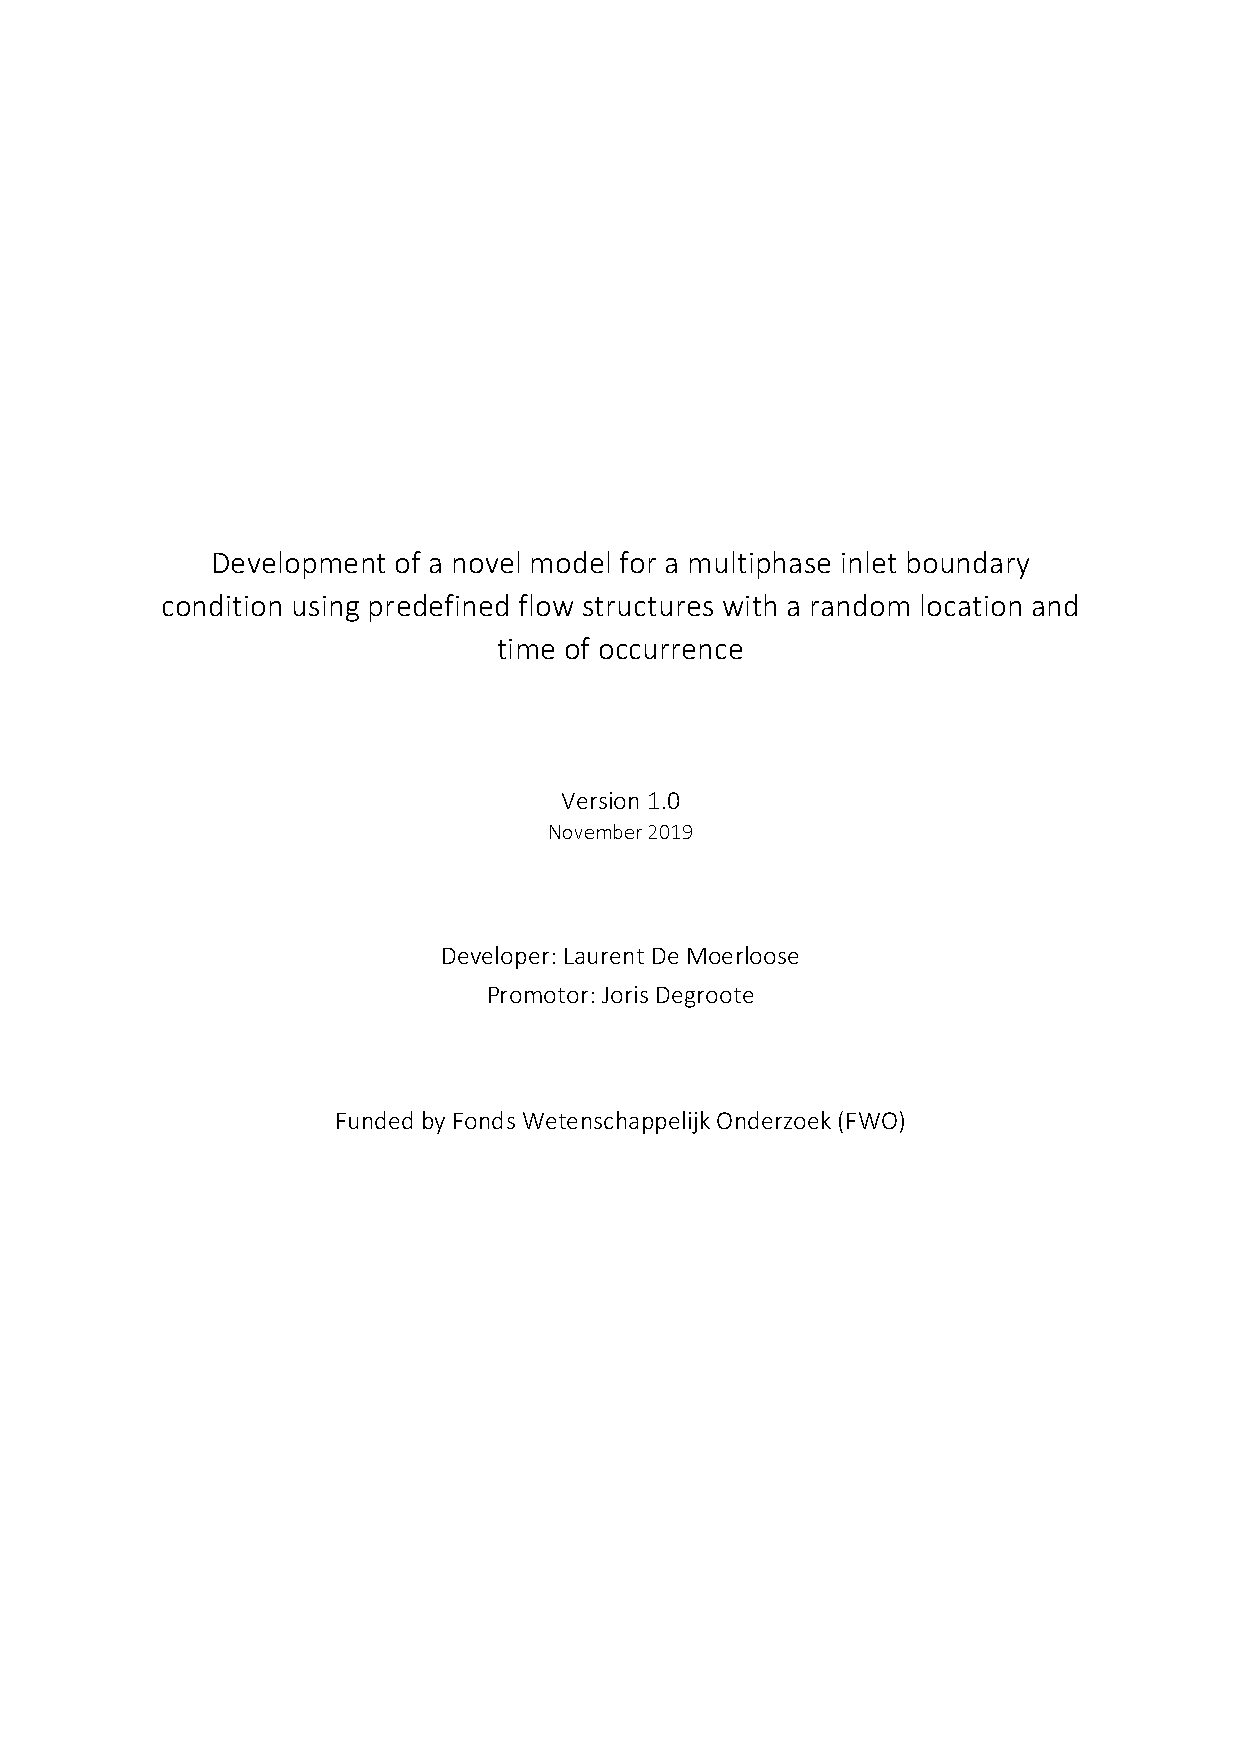
\includepdf{inletModelling_voorblad.pdf}
\frontmatter
\section*{Introduction \label{introduction}}
Within the framework of the Ph.D. of Laurent De Moerloose, it was shown that the modelling of boundary conditions is even more critical in multiphase flow than it is in single-phase flow. This is due to the fact that a slight modelling error can cause an unphysical distribution of the phases. Especially when using fluids with significantly different densities (e.g. air-water mixtures) in a mixture model (such as Volume-Of-Fluid or Level-Set), the maldistribution of the heavier phase possibly leads to larger acceleration terms in the momentum equation, which again leads to large pressure gradients in the flow. The need for implementing a physically accurate inlet model in mixture model simulations is large, but in literature little research about boundary conditions in numerical simulations of two-phase flows can be found. Most papers discuss Lagrangian particles. The Eulerian-Lagrangian model is appropriate for small spherical bubbles, but becomes unreliable for larger bubbles (in which simple closure models for lift, drag, buoyancy and impact forces do not suffice). Another approach for flows with small bubbles is to not explicitly model the bubbles, but to assume a homogeneous distribution such that a single-phase flow model with altered fluid conditions is sufficiently accurate.
\par The Ph.D. of Laurent De Moerloose discusses numerical simulations of air-water mixtures through a number of geometries. The main focus is the quantification of the vibrations of the surrounding structure due to the internal or external two-phase flow. As such, mostly slug, churn and intermittent flow regimes are of importance, as many sources in literature confirm that the largest vibration amplitudes occur in these flow regimes. Lagrangian tracking or not explicitly modelling the gas bubbles is not an option in these flow regimes. One can define an inlet condition with a certain preset and constant distribution of liquid and gas, but in slug flow conditions the continuous gas layer has to be broken up somewhere in the domain. Although physical instabilities can arise, the break-up of the gas layer might just as well be caused by purely numerical (unphysical) instabilities. The subsequent bubble distribution is not necessarily physically accurate. Moreover, in vertical flows, the interface close to the inlet can become oddly shaped, typically prior to calculation divergence. 
\par Therefore, it was concluded that a new type of inlet model should be defined in order to make the results of the subsequent simulation both more accurate and computationally stable. The following characteristics were desired for the new model:
\begin{itemize}
	\item{\textit{Transient}: The gas should enter the domain in predefined bubble shapes, not as a continuous jet with constant velocity and cross-section.}
	\item{\textit{Eulerian}: Large gas bubbles are most important with respect to forces exerted on the surrounding structure. The inlet model should therefore allow the occurrence of large bubbles.}
	\item{\textit{Arbitrary shapes}: Both spherical and non-spherical bubble shapes should be defined.}
	\item{\textit{Random occurrence}: Two-phase flows are inherently not periodic. Therefore, the model should contain some level of randomness: the occurrence of bubbles - with preset shapes - should be randomized. Also the choice between the predefined shapes should be random.}
	\item{\textit{Solver-independent}: Although inevitably the designed model should be able to read and write files in a format specific to the desired flow solver, the actual modelling part of the code should remain independent of the flow solver to be used in the subsequent simulation.}
\end{itemize}
\par This model has been subdivided in three parts, as will be discussed in \mbox{Section \ref{schematic}}. These three parts are defined in separate files and were coded in Python \mbox{Anaconda (\textit{.py})}. The serial execution of the Python-scripts and the definition of case-dependent variables are contained in a bash \mbox{script (\textit{.sh})}. The separate parts of the inlet model are described in \mbox{Section \ref{subparts}}.
\tableofcontents
	

%% THE DOCUMENT ITSELF   %%
%%%%%%%%%%%%%%%%%%%%%%%
\mainmatter     % related to chappg numbering
\raggedbottom % To prevent rubber spacing, so that paragraphs are spread out uniformly over a page causing large spaces between them
\selectlanguage{english}
\renewcommand*{\thesection}{\arabic{section}}

%\newcommand\fdtsvrightmarktmp{{\scshape\small Chapter }}
%\renewcommand\evenpagerightmark{{\scshape\small\chaptername\ \thechapter}}
%\renewcommand\oddpageleftmark{{\scshape\small\chaptername\ \thechapter}}
%\renewcommand\oddpageleftmark{{\scshape\small\leftmark}}

%\addtolength{\headwidth}{\marginparsep}
%\addtolength{\headwidth}{\marginparwidth}

\newcommand{\tm}[1]{$\mbox{#1}^{\mbox{\emph{\scriptsize TM}}}$}

\baselineskip 13.0pt

% Setting headers and footers
\fancyhf[EH]{}
\fancyhf[OH]{}	
\fancyhf[OHR]{\rightmark}
\fancyhf[FC]{\thepage}
\fancyhf[EHL]{\rightmark}

%\hyphenpenalty=5000 %damned hyphenation
%\exhyphenpenalty=5000

% Actual text
\section{Schematic overview of the model\label{schematic}}
A schematic overview of the complete inlet model is shown in \mbox{Figure \ref{fig-schematic}}. The user input is defined in the bash script \textit{masterscript.sh}, which will be discussed in further detail in \mbox{Section \ref{subparts-master}}. The actual modelling is done in three separate Python-files, which have to be executed in sequence. The first script, \textit{readInlet.py} (see \mbox{Section \ref{subparts-reading})}, reads the case-specific inlet geometry for which a model will be developed. Subsequently, the script \textit{inletModelling.py} (see \mbox{Section \ref{subparts-model})} is executed. The actual boundary condition modelling is performed here. Finally, the script \textit{writeBC.py} (see \mbox{Section \ref{subparts-writing})} is used to write the modelled inlet to another file format readable by the flow solver to be used in the simulation which normally follows the inlet modelling stage. The Python-files are called from within the aforementioned bash-script. The scripts used for reading the geometry and writing the modelled inlet are flow solver-dependent, but the actual inlet modelling -defined in \textit{inletModelling.py}- is independent from the flow solver to be used for mesh generation and/or numerical calculation. 
\begin{figure}[h!]
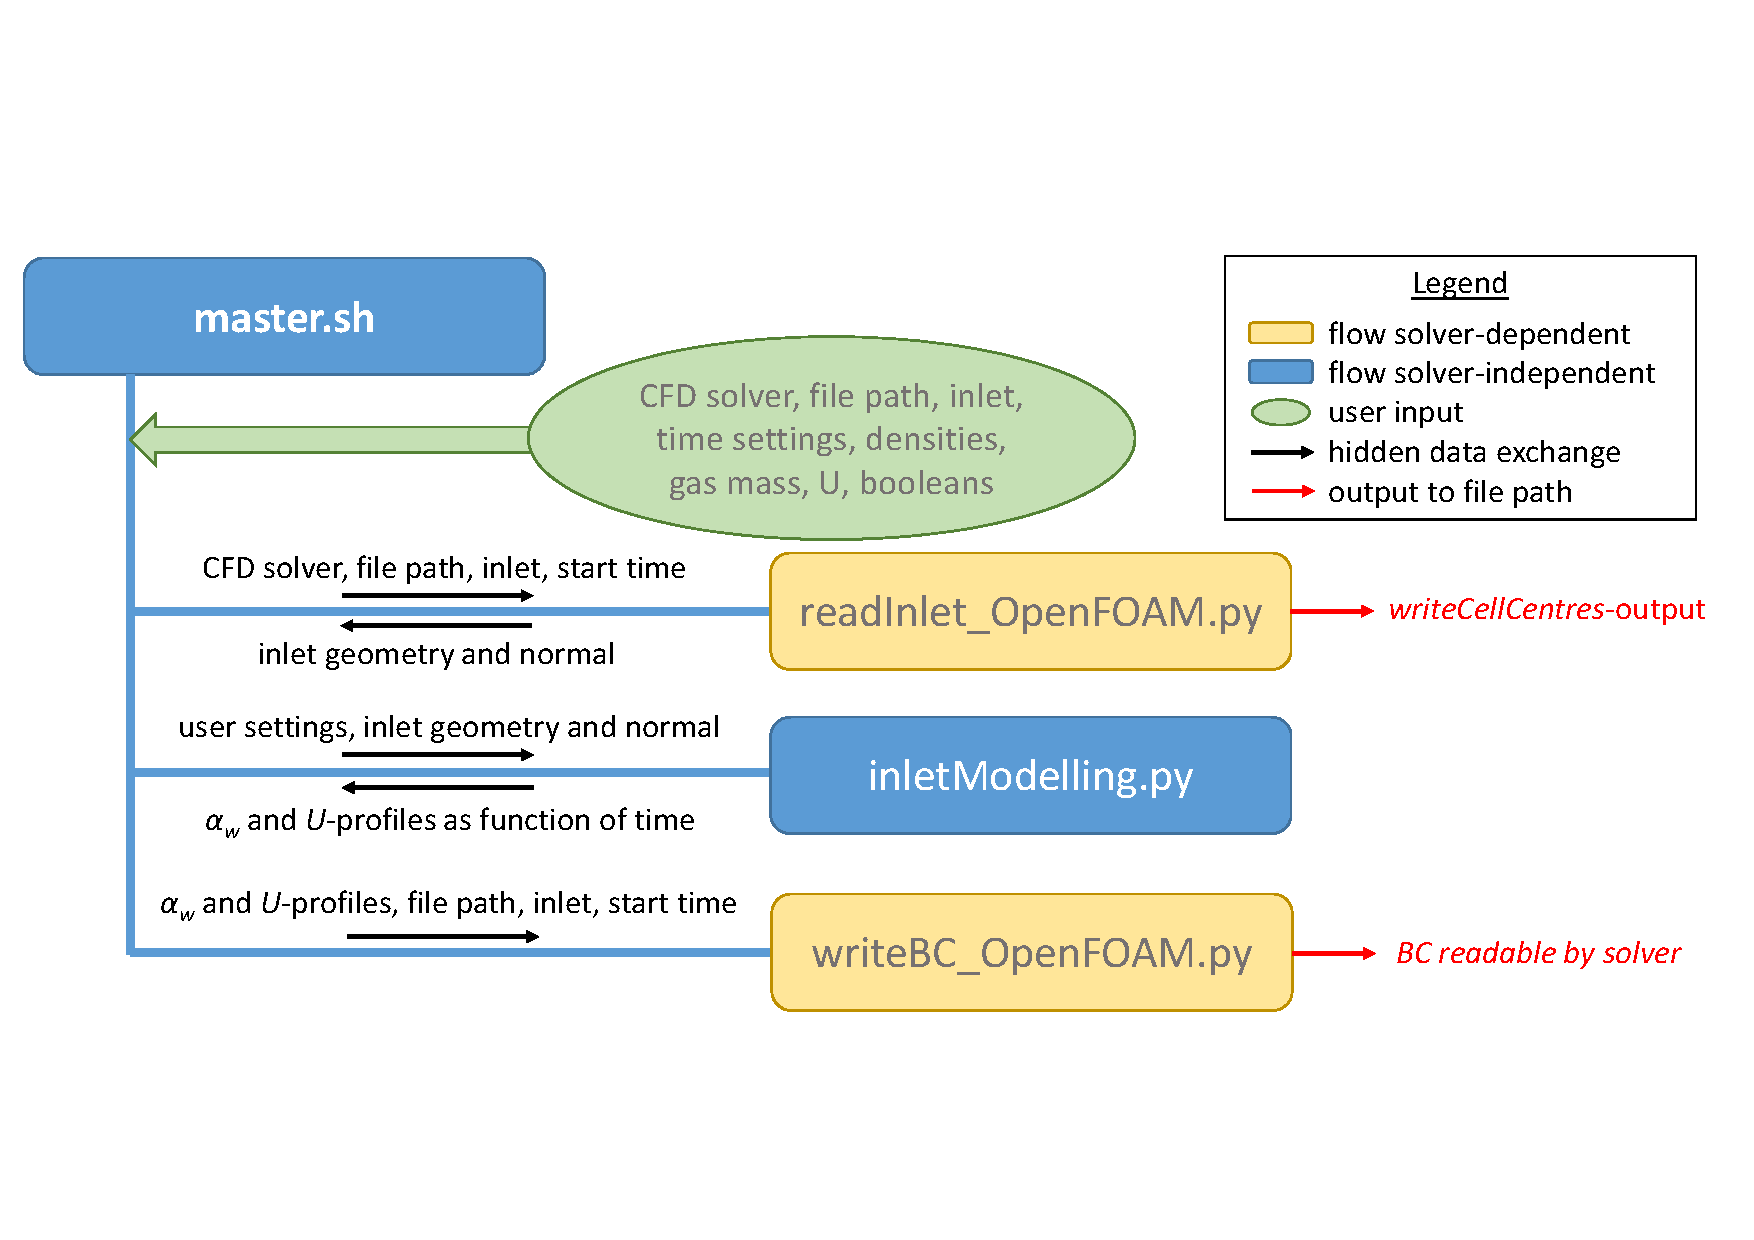
\includegraphics[width=\textwidth,trim={0cm 3cm 0cm 3cm},clip]{inletModelling_schematic.pdf}
\caption{Schematic overview of the complete inlet modelling script. The user input is contained within a master \textit{.sh}-script, which also handles the communication between subsequent steps of the model defined in \textit{.py}-scripts. \label{fig-schematic}. }
\end{figure}
\section{Description of the subparts of the model \label{subparts}}
The inlet modelling code consists of a number of subparts which have been mentioned in the previous paragraph. In this section, these subparts - which are defined in separate files - are discussed in more detail. The code was devised to be comprehensible to people who want to adapt it in a later stage, so each script-file contains both a brief introduction at the top and several comments throughout the code. Therefore, the discussion below will be kept rather general; for the practical implementation, the user is referred to the code itself.
\subsection{Master script (.sh) \label{subparts-master}}
The master file is a short bash script which can be divided in two parts: the first one contains all the variable definitions which are required for the model to work, i.e. the user input. For users who are satisfied with the code as it is and just want to use the model as a black-box, this is the only part of the code that has to be changed. The user input variables are listed below:
\begin{itemize}
	\item{\textit{CFD\textunderscore PROGRAMME}: The flow solver that was used for mesh generation and that will be used for subsequent simulations. In the current version, it is assumed that prior mesh generation and posterior numerical simulation are performed in the same solver, although this can easily be adapted by splitting this variable into two separate parameters.}
	\item{\textit{CFD\textunderscore VERSION}: Version of the flow solver defined in \textit{CFD\textunderscore}\newline\textit{PROGRAMME}. The module of the flow solver is constructed as follows: \textit{CFD\textunderscore PROGRAMME/CFD\textunderscore VERSION}.}
	\item{\textit{PYTHON\textunderscore VERSION}: Name of the Python-module to be loaded.}
	\item{\textit{DIM}: Number of spatial dimensions of the domain. This can be either 2 or 3.}	
	\item{\textit{CASE\textunderscore PATH}: Full path where the CFD case is defined. This does not need to be the location from where the script is executed. However, it is necessary that all files comprising the model are located in the same folder, from where the master script (see \mbox{Section \ref{subparts-master}}) is executed, which does not need to be the case path.}	
	\item{\textit{startTime} [$\mathrm{s}$]: Value of the first time step for which the inlet needs to be modelled. In OpenFOAM, the corresponding time step folder has to exist prior to the execution of this model.}
	\item{\textit{endTime} [$\mathrm{s}$]: Value of the last time step for which the inlet needs to be modelled.}
	\item{\textit{timeStepSize} [$\mathrm{s}$]: Value of the time step used in the inlet model. }
	\item{\textit{tunit} [$\mathrm{s}$]: Model parameter. In this model, the total time interval defined by the start and end time, are divided in subintervals of length \textit{tunit}. It is necessary (and explicitly checked upon execution of the model) that \mbox{(\textit{endTime} -\textit{startTime})} is a multiple of \textit{tunit}. During each subinterval of size \textit{tunit}, the model introduces a given mass of gas defined in \textit{mg} (see further). As such, a low value of \textit{tunit} leads to a more regular distribution of the gas over time. A high value of \textit{tunit} possibly leads to the existence of large and irregularly distributed bubbles. }
	\item{\textit{inletName}: Name of the inlet boundary to be modelled. This name has to correspond with the name given to the inlet during mesh creation.}
	\item{\textit{rhog} [$\mathrm{kg/m^3}$]: Density of the gas. }
	\item{\textit{rhol} [$\mathrm{kg/m^3}$]: Density of the liquid (actually not used in the current version of the model, but further refinement of the model might require the definition of this variable). }
	\item{\textit{mg} [$\mathrm{kg}$]: Mass of gas to be introduced during a time interval denoted by \textit{tunit} (see earlier). }
	\item{\textit{tol\textunderscore mg} [$\mathrm{kg}$]: Absolute tolerance on the amount of gas introduced per time interval \textit{tunit}. The model jumps to the next time interval whenever the amount of gas actually introduced in the current time interval is within \textit{tol\textunderscore mg} of the desired \textit{mg}. }
	\item{\textit{U} [$\mathrm{m/s}$]: Flow velocity normal to the inlet plane. Currently, as no slip between the phases is modelled, this velocity value does not change. However, it is already included in the model framework in order to provide an easier implementation of interphase slip in future developments. }
	\item{\textit{intersectBoundary}: Boolean indicating whether a bubble is allowed to intersect with a boundary adjacent to the inlet boundary. If set to \textit{True}, the bubble is allowed to intersect with a boundary, which means that some part of the modelled bubble will be cut off. The model automatically calculates how much mass was actually added. If set to \textit{False}, only whole bubbles can be introduced, but the zones next to side or internal walls will have a low gas void fraction, if not zero.}
	\item{\textit{intersectBubble}: Boolean indicating whether a bubble is allowed to intersect with a bubble that has already been defined by the model. If set to \textit{True}, the bubble is allowed to intersect with a bubble, which means that some part of the modelled bubble will be cut off. The model automatically calculates how much mass was actually added. This possibly leads to unphysical shapes, however. If set to \textit{False}, the bubbles can at most touch each other in the final inlet profile. }
\end{itemize}
\par In the second part of the script, the three Python-files are called in sequence. The \textit{readInlet}- and \textit{writeBC}-scripts are solver-dependent. Currently, these were only defined for OpenFOAM. The script checks beforehand what flow solver was defined through an \textit{if}-statement, so that if a user wants to use another solver, the adapted scripts can be added to the \textit{if}-statement with minor adjustments.
\subsection{Reading the inlet geometry (.py) \label{subparts-reading}}
This script reads the cell center locations of the cells located at the inlet, i.e. it reads the inlet geometry. Currently, only the OpenFOAM-version was defined. As this is naturally solver-dependent, this script will have to be adapted if another flow solver is requested.
\par In the OpenFOAM version, the OpenFOAM-utility \textit{writeCellCentres} is called; this function writes the cell center coordinates in separate files (\textit{ccx} for the x-coordinate, \textit{ccy} for the y-coordinate and \textit{ccz} for the z-coordinate), as well as the face areas on the boundaries of the domain (\textit{V}, which contains the  cell volumes for the internal field as well). Subsequently, the Python-code looks for the name of the boundary (given as user input) inside these files to locate the inlet geometry. Only the inlet coordinates and face areas are read by the Python-code and stored in a numpy-array called \textit{coordList}. This array consists of 5 columns: cell id (which is just a list of natural numbers ranging from 0 to the number of cell centers located at the inlet), x-coordinate, y-coordinate, z-coordinate and face area. Exception handling has been implemented because it is possible that the inlet has a uniform value in one dimension. In that case, OpenFOAM stores that coordinate as a single uniform value and not as an entire list. This is taken care of in the \textit{except}-clause.
\par In the final step of the Python-script, the normal to the inlet face is calculated from the coordinates list. This normal is defined as the normal pointing into the domain and is required for the correct bubble definition in the \textit{inletModelling}-script. In case of a three-dimensional case, the normal is automatically calculated from three non-linear points in the inlet face, without additional user input. In case of a two-dimensional case, the script asks the user for the coordinates of the vector normal to the inlet. Both the normal and the coordinates list are saved in \textit{.npy}-files, which are not removed after completion of the script to allow for easy manual checks if desired by the user.
\subsection{Modelling the inlet boundary condition (.py) \label{subparts-model}}
The \textit{inletModelling}-script is the core of the inlet model. It has been made solver-independent deliberately, such that the actual inlet modelling can be used for any flow solver (after altering the \textit{readInlet}- and \textit{writeBC}-scripts, naturally). Fundamentally, this script initializes two matrices in which each row (dimension 0) corresponds to a cell located at the domain inlet and in which each column (dimension 1) corresponds to a time step in which the inlet condition has to be modelled. One matrix corresponds to the velocity $U$, which is a vector field. The second matrix defines the volume fraction of water inside each cell, $\alpha_{w}$. The matrices are initialized with the values for pure liquid: $U$ contains the liquid velocity and $\alpha_{w}$ contains 1 in each cell.
\par This core script can be subdivided in two parts. The first part (which is defined near the end of the script) consists of a \textit{for}-loop, which is executed for each interval to be defined. An interval is defined as the difference between end and start time, divided by the parameter $t_{unit}$. It is checked that this ratio is an integer value. Inside each interval, a total amount of mass $mg_{tunit}$ should be introduced, distributed over bubbles of different size, shape and location. While the requested amount of gas is not attained, new bubbles are introduced. Each iteration of that \textit{while}-loop corresponds to the (attempted) definition of a new bubble. The location and size of that bubble is chosen randomly; the bubble shape is chosen randomly from the predefined list of arbitrary shapes (currently, only one shape is defined). It is possible, especially with the random character of the bubble parameters, that a bubble cannot be defined for the given settings. In that case, the script ends the current iteration without changing anything to the $U$ and $\alpha_{w}$-matrices and goes to the next iteration, in which new bubble parameters will be chosen. If a number of iterations is reached without insertion of a new bubble, the script is stopped and the user is informed that it was not possible to define an inlet boundary condition with the given user-defined settings. This number is hard-coded to 1000. When the bubbles inside an interval have been defined successfully, the code goes to the next interval, until the entire time range between start and end time has been defined.
\par The second part of the script is defined in the function \textit{bubbleShape}, which comprises an \textit{if}-statement which operates as a switch between the predefined bubble shapes. In each option of that switch, a fixed shape is defined mathematically. Currently, only one bubble shape is defined, which is a spherical bubble. Whereas the bubble shape is fixed, the bubble size is changeable; the shape is scaled with a factor \textit{mgb} - a variable given to the \textit{bubbleShape}-function - from which the bubble size is determined. The bubble center coordinates and time instant are also given as input to the function, which then evaluates all locations in space and time to define the complete bubble. The bubble location in time cannot be as such that the bubble intersects with the next time interval; this is also checked explicitly inside the function. This effect can be limited by increasing the variable $t_{unit}$, which decreases the number of time intervals. As such, $t_{unit}$ is a parameter which indicates the regularity of the bubbles occurring at the inlet.   The values in the $U$- and $\alpha_w$-matrices are changed for every point defined in the matrix - specified by its spatial coordinates and time instant - which falls within the bubble. In the first version of the code, the bubble speed $U$ is the same as the velocity of the surrounding liquid (so $U$ only consists of uniform values). The value for $\alpha_{w}$ corresponding to a point located inside the bubble, is set to 0. Finally, the \textit{bubbleShape}-function stores the altered $U$- and $\alpha_{w}$-matrices and returns a boolean indicating whether the bubble was introduced correctly and the amount of gas that was introduced (which can differ from \textit{mgb} because of the discrete nature of the mesh).
\par The value of \textit{mgb} is set randomly, but it is checked inside the \textit{bubbleShape}-function whether this value falls in a certain range. The specified range should be bubble-dependent (as some bubble shapes are only physically possibly when they are relatively small or large). Additionally, it is checked whether the amount of gas that is still required (to match the user input variable \textit{mg}) is smaller than the minimal value for \textit{mgb}. In order for the model to be accurate, this has to be defined for at least one bubble shape (and it makes sense that this is done for the spherical shape). If the minimal value \textit{mgb} is larger than the amount of gas that has to be modelled, \textit{mgb} is set to the required amount of gas. In that way, the amount of gas sent through the inlet is exactly equal to what the user-specified, except for a numerical accuracy error related to the discrete nature of the numerical mesh. If a new bubble shape were to be defined, it would not be necessary to incorporate this option in the new bubble shape definition. However, at least one bubble shape should have this option in order to be able to match the value of $mg_{tunit}$ as closely as possible. In the end, the script guarantees the introduction of an amount of gas equal to the user-specified variable, accurate up to an absolute tolerance equal to $tol_{mg}$, which is also set by the user.
\par This script asks for two booleans (which are defined in the master script, see \mbox{Section \ref{subparts-master}}), i.e. \textit{intersectBoundary} and \textit{intersectBubble}. The former confirms whether the bubble can intersect with a boundary (e.g. a wall at the sides of the inlet), the latter whether the bubble can intersect with a previously defined bubble. In both cases, a boolean value "True" indicates that the intersection is allowed.
\par Both the $U$ and $\alpha_{w}$-profile are saved in \textit{.npy}-files, which will be read in the \textit{writeBC}-script. Additionally, both profiles are saved in \textit{.csv}-files, which can be read into ParaFoam for easy visualization of the inlet profile as a function of space and time. 
\subsection{Writing the inlet boundary condition (.py) \label{subparts-writing}}
In this final Python-script, the inlet which has been defined and stored in \textit{.npy}-files in the previous step, are converted into files which are readable by the flow solver. This makes this script solver-dependent. Currently, only the OpenFOAM-version has been modelled and the current description is only applicable to that particular script. 
\par In order to use the inlet model appropriately in OpenFOAM, the boundary condition of $U$- and $\alpha_{w}$-fields at the inlet should be \textit{timeVaryingMappedFixedValue}. The code explicitly checks whether this is the case and exits with a clear error message if the boundary condition was not adapted. The condition \textit{timeVaryingMappedFixedValue} requires the definition of a folder \textit{boundaryData} in the \textit{constant}-folder. The folder \textit{boundaryData} contains a folder with the same name as the inlet boundary (so, typically ``inlet"). The modelled boundary condition for $U$ and $\alpha_{w}$ should be stored here. Firstly, a file called \textit{points}, which is a list of points in space where the flow variable values are set, is created. Note that as the boundary condition name contains the word ```mapped", this list of points does not need to be the full list of nodes located at the inlet. Rather, the \textit{points}-file comprises an arbitrary number of locations where the flow parameter value is set (see further). In this specific case, however, the boundary condition is defined for all cell centres located at the inlet, so the list of points exactly matches the definition of the mesh at the inlet. The actual values of the flow variables $U$ and $\alpha_{w}$ are found in time step folders which are defined in \textit{constant/boundaryData/inlet} as well. Each time step folder contains two files, \textit{U} and \textit{alpha.water}, in which the flow parameter values are set. For example, the vector defined on line 50 in the file \textit{U} corresponds to the value of $U$ to be set at the given time instant and at the location indicated by the coordinates listed on line 50 of the aforementioned file \textit{points}.
\par All files and folders described in this section are constructed with default Python file handling commands. The typical OpenFOAM-file header and footer are defined in separate Python-functions, which are called at the beginning and at the end of the writing process, respectively.
\section{Frequently asked questions about the current version}
\subsection{The code randomly selects a location for the centerpoint – can you implement another distribution than the uniform distribution you implicitly use now?}
Yes, but it is not implemented in the current version. You could use a pseudo-random selector which has a normal distribution and then link the randomly-selected value to a cell ID. For example, if you randomly select a value in a normal distribution between 0 and 1, the value 0.5 could be linked to a cell ID which is the most probable. However, this is quite tedious and probably not very user-friendly. Another way you can do this is keep the same random generator, but beforehand adapt the list of cells you can choose from and duplicate more likely cells. For example, the more likely location can appear twice or more times in the cell selection list, from which then you randomly select a variable in a uniform way. 
\subsection{Can you only define bubbles at locations such that the bubble does not intersect with the wall?}
There is no fundamental reason why bubble and wall intersection should not occur, but you have space to define the restrictions of bubble location inside each bubble shape in the inlet modelling script (not only with regard to the wall boundary but also other arbitrary requirements, if need be). A user-defined boolean in the code determines whether or not bubble-wall intersection is possible. If it is possible, a control loop is needed to determine how much of the bubble was actually defined (because not the entire bubble is modelled) and this amount of gas mass is returned to the main loop in order to get the correct amount of gas you desired within a time range $[0, tunit[$.
\subsection{Can you only define bubbles at locations such that the bubble does not intersect with another bubble?}
It is explicitly checked during the definition of a new bubble that the new bubble does not overlap with a previously defined bubble. This is defined as such: all VOF-values of water which are adapted should be equal to one, which means that the cells were initially filled with water. The idea behind this is that having overlapping bubbles creates a very unphysical shape as the gas will immediately try to adapt its shape to a state with lower surface energy. The unrealistic shape and the possibly strong acceleration of liquid and gas during shape adaptation in the domain might cause instabilities and ultimately divergence in the solver. This, however, is not a limitation, as one can define an arbitrary shape of bubble in the inlet modelling Python-script. Whether two bubbles can intersect is again determined with a user-defined boolean. 
\subsection{How do you add a new bubble shape?}
The bash-script calls three different Python scripts: one to read the inlet geometry, one to model the inlet boundary condition and one to write the inlet boundary condition in a format compatible with the solver. The inlet modelling Python script (the second one) is flow-solver independent and contains all information about the modelling, thus also the bubble shapes. These are defined in a function called “bubbleShape” . You also need to adapt the hard-coded counter ‘nShapes’, which keeps track of the number of defined bubble shapes.
\section{Future steps}
The first version of this model provides a framework which allows the definition of more accurate models to be applied at the inlet. If the user finds experimental data showing the bubble shape and/or size distribution in a specific geometry, this distribution can be modelled within the current framework. However, a number of steps can still be made to increase the accuracy and the range of this model. Two improvements are proposed below.
\subsection{Improving model accuracy}
\par Currently, the speed of the gas bubbles is the same as that of the surrounding liquid. This is chosen in such a way because of predicted stability issues: a sudden increase in velocity when a bubble enters the domain, especially in an incompressible flow, might trigger high pressures and even divergence of the calculation. However, modelling the slip between both phases will naturally increase the accuracy of the model, as well as reduce the domain length (currently, if slip is desired, still a small precursor domain is required in order for buoyancy to have an effect and to create slip). This is a natural next step in the improvement of this model. As argued before, this might require more accurate wake modelling to avoid numerical instability. This could be implemented by changing the liquid speed upstream and downstream of the bubble as well, i.e. to come closer to an actual wake modelling. 
\par Another improvement is related to bubble shape definition. On the one hand, it is obvious that the true strength of this script is the possibility to define arbitrary bubble shapes. Case-dependent bubble shapes, such as bubbles taking the shape of the gap in between different pipes in a tube bundle, can easily be added to the inlet modelling script. On the other hand, the bubbles are currently defined in a binary way: the cell value of $\alpha_{w}$ is either 0 or 1. For better interface representation, the model could be extended to yield intermediate values. It must be mentioned that the Volume-Of-Fluid method stabilizes the interface through (numerical) diffusion and automatically yields intermediate values of $\alpha_{w}$ in the first time steps of the simulation. Therefore, this proposed improvement is not about numerical stability, but purely about accuracy improvement. This being said, the same numerical diffusion also renders a more accurate interface modelling moot to some extent. Significant attempts have been made to improve interface modelling in scientific literature, but these studies are of more fundamental nature (typically a domain containing only one bubble, not related to vibrations or heat transfer applications). These studies use very fine meshes close to the bubble interface, which is at the given time not feasible for applications of larger scale, which was the framework in which the model was developed.  Arguably, in the latter applications, the exact shape of the interface is of lesser importance. The relevance of the proposed change should consequently be evaluated based on the application.
\subsection{Improving model efficiency}
The current version has not been implemented in the most efficient way. During the development of this model, the emphasis was not on efficiency, mostly because two-phase flow simulations take considerable time to complete and therefore the inlet model was not deemed to be the most time-critical step in the total simulation time. Admittedly, this does not hold for simple cases with coarse meshes, especially in certain ranges of the inlet model's parameters as shown with the 3x5 tube bundle test case. Some improvements towards a more efficient model can be given.
\par Firstly, for every newly defined bubble, all cells in the virtual precursor domain (the two-dimensional inlet geometry combined with the total unit time to be modelled) are checked to verify whether a given cell is located inside the bubble or not. Reducing the unit time will reduce the computational time of this step but also limits the maximum achievable bubble size. The modelling time can be drastically reduced without limiting the modelling capabilities such as bubble size. The current method is equivalent to a brute force search algorithm. In computer science literature, a lot of different faster search algorithms can be found. Consequently, coding a smarter search algorithm into the inlet model might be beneficial.
\par Another flaw of the code is that it only checks whether the boundary cuts the bubble after definition of the bubble into a temporary matrix. This means that the code has looped over all cells of the virtual precursor domain before evaluating whether the bubble's location is acceptable or not. It would be more efficient to check the bubble-wall intersection beforehand. However, two problems are encountered when trying to do this. The first problem is that the geometrical definition of a random OpenFOAM-case is lacking. The mesh boundaries are defined as a set of faces and these are defined as a set of edges, which are a set of points. Finding the exact location of the walls is therefore possible, but requires looking up all the OpenFOAM-files in Python which is very tedious to code. Afterwards, one will have to cross-check these boundary nodes with the inlet face nodes to see which inlet nodes are part of the walls. Indeed, the calculation becomes more efficient because one can hence easily check whether such a node would be inside the bubble. However, and this is the second problem, one still needs to check whether the newly defined bubble does not intersect with an old bubble and for that a loop over all nodes located inside the bubble is needed. This means that all nodes located inside the new bubble have to be known at this point and this means that the current control mechanism occurring after the bubble definition still needs to be present. So, overall, the computational time gain will be limited compared to the time it takes to recode the Python algorithm but also compared to the time it takes to define the wall BC for each case separately.
In other words, in the general case, it is best to keep the rigorous check of all cells inside the bubble to determine whether the bubble intersects with a wall. But, for a specific case – if you want to repeat the same geometry over and over again –  the current version of the code does allow the introduction of additional requirements that the chosen bubble location should have. If these requirements are not met by the randomly chosen position, the bubble is not inserted and a new position is chosen by the Python script’s random generator, before all node positions are compared to the bubble center's location. So, the current model already has an option to make this script run more efficiently than it does in the general case, but this option has to be modified on a case-per-case basis.
\section{Final note}
It is my hope that the inlet model will be used in other applications of the Volume-Of-Fluid method. What improvements and changes, if any, need to be done, will be determined largely by the specific application and specific demands set by the user. In that way, this code will hopefully be a stepping stone for future researchers.

\end{document}
